\documentclass[a4paper,UTF8]{article}
\usepackage{ctex}
\usepackage[margin=1.25in]{geometry}
\usepackage{color}
\usepackage{graphicx}
\usepackage{amssymb}
\usepackage{amsmath}
\usepackage{amsthm}
\usepackage{booktabs}
\usepackage{caption}
\usepackage{fancyhdr}
\usepackage{extramarks}
\usepackage{amsfonts}
\usepackage{tikz}
\usetikzlibrary{arrows}
\usepackage{algorithm}
\usepackage{algorithmicx}
\usepackage{algpseudocode}
\usepackage{listings}

%\usepackage[thmmarks, amsmath, thref]{ntheorem}
\theoremstyle{definition}
\newtheorem*{solution}{Solution}
\newtheorem*{prove}{Proof}
\usepackage{multirow}

%
% Basic Document Settings
%

\topmargin=-0.45in
\evensidemargin=0in
\oddsidemargin=0in
\textwidth=6.5in
\textheight=9.0in
\headsep=0.25in

\linespread{1.1}

\pagestyle{fancy}
\lhead{\hmwkTitle}
\chead{\hmwkClass\ (\hmwkClassInstructor\ \hmwkClassTime)}
\rhead{\hmwkAuthorName}
\lfoot{\lastxmark}
\cfoot{\thepage}

\renewcommand\headrulewidth{0.4pt}
\renewcommand\footrulewidth{0.4pt}

%
% Homework Details
%   - Title
%   - Due date
%   - Class
%   - Section/Time
%   - Instructor
%   - Author
%

\newcommand{\hmwkTitle}{Assignment \ \#4}
\newcommand{\hmwkDueDate}{October 5, 2017}
\newcommand{\hmwkClass}{Problem Solving}
\newcommand{\hmwkClassTime}{}
\newcommand{\hmwkClassInstructor}{Professor Chen}
\newcommand{\hmwkAuthorName}{李志琦 161220074}

%--

%--
\begin{document}


\subsection*{7.1}
\subsubsection*{a}
suppose D is not strong, so there are two vertices $m,n$, s.t there is a $m~n$ path
,but there isn't a $n-m$ path, so we choose another vertex v(neight m or n). if we remove v,so
D-v is not strong because there is not a $n~m$ path. So D is strong.
\subsubsection*{b}
if a graph C od order 3 is strong, so it must be a circle like this.

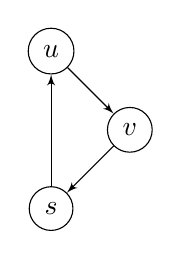
\begin{tikzpicture}
\tikzset{vertex/.style = {shape=circle,draw,minimum size=0.5em}}
\tikzset{edge/.style = {->,> = latex'}}
% vertices
\node[vertex] (s) at  (0,0) {$s$};
\node[vertex] (u) at  (0,2) {$u$};
\node[vertex] (v) at  (1,1) {$v$};
%edges
\draw[edge] (s) to   (u);
\draw[edge] (u) to   (v);
\draw[edge] (v) to   (s);
\end{tikzpicture}

so if the graph D's 4 vertices is $u,v,p,q$, so if we remove u,v,p  each time
D-u,D-v,D-p is still a strong graph.so these three graphs maybe

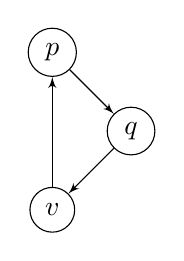
\begin{tikzpicture}
\tikzset{vertex/.style = {shape=circle,draw,minimum size=0.5em}}
\tikzset{edge/.style = {->,> = latex'}}
% vertices
\node[vertex] (v) at  (0,0) {$v$};
\node[vertex] (p) at  (0,2) {$p$};
\node[vertex] (q) at  (1,1) {$q$};
%edges
\draw[edge] (v) to   (p);
\draw[edge] (p) to   (q);
\draw[edge] (q) to   (v);
\end{tikzpicture}
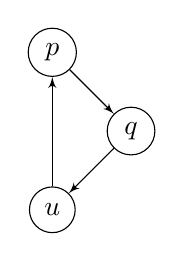
\begin{tikzpicture}

\tikzset{vertex/.style = {shape=circle,draw,minimum size=0.5em}}
\tikzset{edge/.style = {->,> = latex'}}
% vertices
\node[vertex] (u) at  (0,0) {$u$};
\node[vertex] (p) at  (0,2) {$p$};
\node[vertex] (q) at  (1,1) {$q$};
%edges
\draw[edge] (u) to   (p);
\draw[edge] (p) to   (q);
\draw[edge] (q) to   (u);
\end{tikzpicture}
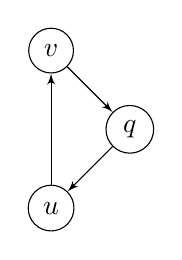
\begin{tikzpicture}

\tikzset{vertex/.style = {shape=circle,draw,minimum size=0.5em}}
\tikzset{edge/.style = {->,> = latex'}}
% vertices
\node[vertex] (u) at  (0,0) {$u$};
\node[vertex] (v) at  (0,2) {$v$};
\node[vertex] (q) at  (1,1) {$q$};
%edges
\draw[edge] (u) to   (v);
\draw[edge] (v) to   (q);
\draw[edge] (q) to   (u);
\end{tikzpicture}

we know the sum of indegree and outdegree of vertex q is 3, is can be 2 in-edge and 1 out-edge of
1 in-edge and 2 out-edge, but each triangle that q lies on will choose two edges that  one incident to
q and another incident from q and every triangle chooses differently. it's impossible because vertex q
can provide at most two different combinations but there are three triangles.

\subsection*{7.2}
if G is Eulerian, we can find a Eulerian circuit and we can assign a direction on tcircuit, and assign each edge a direction, so itis an Eulerian orientation.
\subsection*{7.4}
if digraph D is strong

then for eac pair vertices u,v there is a u-v path and a v-u path.
if we reverse the direction iof every arc of D, so u-v path will be v-u path in $\vec D$ , and v-u path
will be a u-v path in $\vec D$, so for each pair  u,v vertices in $\vec D$, there are both u-v path and v-u path

if digraph $\vec D$ is strong
it's same as we prove above, bacause it's symmetrical

\subsection*{7.5}
1. if D is strong

for any two sets A and B.
then for a vertex in A, a vertex in B, because there is a u-v path, so there is an arc from A to B.
because there is a v-u path, so there is an arr from B to A

2 prove D is strong

D's underlying graph is connected, otherwise D will has morn than two components and obviously impossible.

for each pair vertices u,v in V
firstly, we let A be {u} and let v in B. for any vertices incident to u in B, we add them to A and keep finding the vertices that incident to them. if we find v, stop.
for any vertices incident from u in B, we add them to B and keep finding the vertices that incident from them. if we find v, stop.

we must can find v because (fail to prove it)


\subsection*{7.9}
if toutnament T is transitive:

because there is Hamiltonain path in T $v_1 \to v_2 ... \to v_n $, so if the outdegree of $v_i$ is k then $v_{i-1}$ is at least k+1
because  T is transitive ervery vertex incident from $v_i$ is incident from $v_{i-1}$ and $v_i$ is also incident from $v_{i-1}$
so for each pair vertices $v_i,v_j$ the degree $v_i$ is larger than $v_j$ is i<j

if every two vertices of T has distinct outdegrees.

we just prove that T don't contain Hamiltonain circle use Pigeonhole principle, if T has a Hamiltonain circle then n vertices there outdegree is from 1 to n-1,must has at least two vertices has same outdegree.

so T contains no Hamiltonain circle. so T is transitive


\subsection*{7.10}
the shortest u-v path is folowingf, and the vertives from $v_1$ to v will be incident to u
otherwise the $\vec d$ will be smaller than k. the number of vertices from $v_1$ to v is k-1
so id u $>=$ k-1
$u \to v_1 \to v_2 ... v$

\subsection*{7.13}
min ($\vec d$(u,v),$\vec d$(v,u))
 is 1, and another must be larger than 1, because there is only one between arc(u,v) and arc(v,u)

\subsection*{7.14}

\subsubsection*{a}
if the Tournaments of order 3 contains a Hamiltonain circle. every team can be the champion.
\subsubsection*{b}
first we know in a Trounaments $\sum indrgeee$ and $\sum outdegree$ equals,so if a Trounaments with even order, each vertex has same indegree m,and outdegree n
,because m+n is odd so ,m!=n so  $\sum indrgeee$ != $\sum outdegree$. so it impossible fo all  vertices has same outdegree and same indegree.
\subsection*{7.15}
from Throrem 7.10 we know T has a Hamiltonain circle of length n;

from Throrem 7.11 we know there exists a T-v is a strong Tournament;

from Throrem 7.10 we know T-v has a Hamiltonain circle of length n-1;

....

from Throrem 7.11 we know there exists a tournament $T_3$ of order 4 is a strong Tournament;

from Throrem 7.10 we know $T_3$ has a Hamiltonain circle of length 3;

so we get it.





\end{document}
